\subsection{Cuprates: High temperature superconductors}
\begin{figure}
    \centering
    \begin{subfigure}{0.48\textwidth}
        \centering
        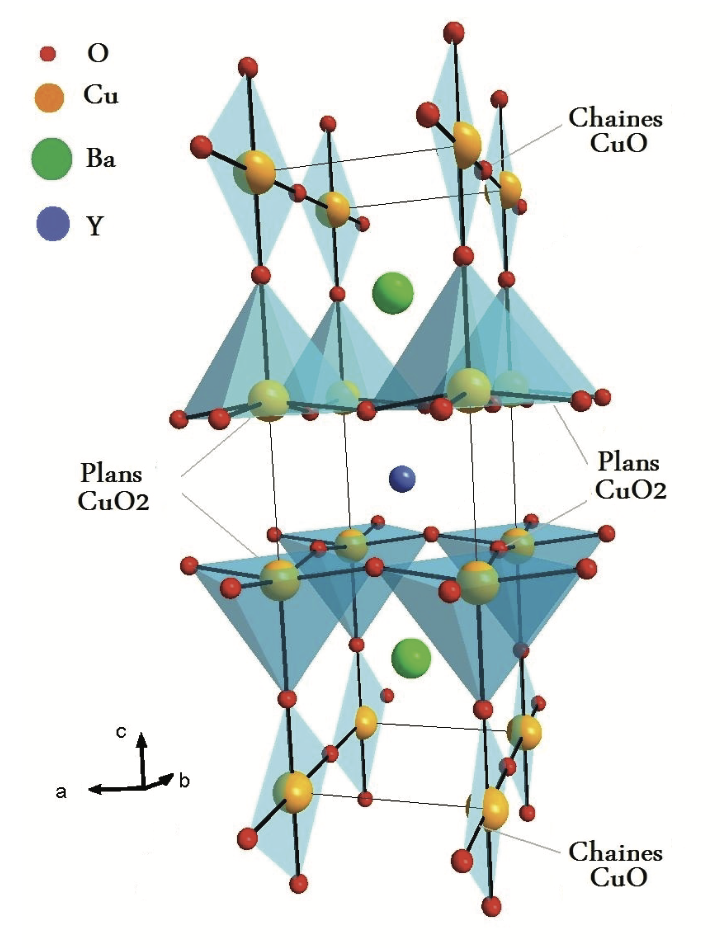
\includegraphics[width=\textwidth]{figures/cuprate_structure}
        \caption{Crystal structure of a Cuprate (YBCO)}
        \label{fig:cuprate_structure}
    \end{subfigure}
    \begin{subfigure}{0.48\textwidth}
        \centering
        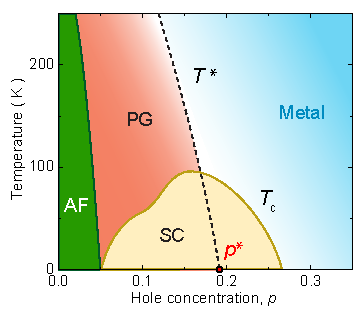
\includegraphics[width=\textwidth]{figures/phase_diagram}
        \caption{Phase diagram of cuprates. $p^*$ marks the QCP.}
        \label{fig:phase_diagram}
    \end{subfigure}
    \caption{Physical description of cuprates.}
\end{figure}

Cuprates are a class of superconductors with high critical temperature that have been subject
to intense research since their discovery in 1986. They exhibit rich physical behavior, specially
in their various phases.

The crystal structure of cuprates is a perovskite structure, with a copper-oxygen plane
($\mathrm{CuO}_2$) as the main conducting layer. This structure is shown in Figure
\ref{fig:cuprate_structure}.